% Machine translated from the Danish original, ../danish/dma-problems-january-2026.tex
\noindent\emph{This problem set has been machine translated from the Danish original.}
\medskip

\multiplechoicestart


\question{Good properties of algorithms}
Which of the following properties are typically desirable for an algorithm?
\multipleanswers
\optionsstart
\answer It runs fast \correct
\answer It mostly uses for loops and no or very few while loops
\answer It uses all of the computer's memory
\answer It makes many recursive calls
\answer It gives the desired result for every possible input \correct
\answer It is hard to understand, so nobody can copy it
\optionsend
\explanation{
Good algorithms are efficient (fast and with low memory usage) and give the desired result in all cases. Using particular control structures, using a lot of memory, or making the algorithm unnecessarily complex are not desirable properties.
}

\question{Probabilities}
Which of the following numbers can be probabilities?
\multipleanswers
\optionsstart
\answer $-2$
\answer $10^{-9}$ \correct
\answer $0.25$ \correct
\answer $1$ \correct
\answer $1.5$
\answer $2$
\answer $-0.5$
\optionsend
\explanation{
A probability is always a number in the interval $[0,1]$. Negative numbers and numbers greater than $1$ cannot be probabilities.
}

\question{Number of sequences}
We have 10 different playing cards in a hat. We draw a card and put it back, and we do this 5 times. How many different sequences of 5 cards are possible?
\oneanswer
\optionsstart
\answer $5^{10}$
\answer $\binom{10}{5}$
\itxanswer{binom(10,5)}
\answer $5!$
\answer $10!$
\answer $10^5$ \correct
\optionsend
\explanation{
In each of the 5 draws there are 10 possible cards.
The number of possible sequences is therefore $10^5$.
}

\question{Properties of graphs}
Which of the following words describe properties of graphs?
\multipleanswers
\optionsstart
\answer connected \correct
\answer harmonic
\answer isotropic
\answer directed \correct
\answer projective
\answer acyclic \correct
\optionsend
\explanation{
Typical properties of graphs are connected, directed and acyclic.
}


\question{Basic pseudocode keywords}
Which of the following words do we often use in basic pseudocode?
\multipleanswers
\optionsstart
\answer so
\answer must
\answer prioritize
\answer else \correct
\answer while \correct
\optionsend
\explanation{
Pseudocode uses control structures such as while and else.
We do not use the other words in pseudocode.
}


\question{Data structures from the syllabus}
Which of the following words are names of data structures from the course syllabus?
\multipleanswers
\optionsstart
\answer index tree
\answer stack \correct
\answer heap \correct
\answer container
\answer hyperlist
\answer group
\optionsend
\explanation{
In the course we have learned about stacks and heaps.
The other words are not standard data structures.
}

\question{Properties of max-heaps}
Which of the following statements hold for every max-heap?
\multipleanswers
\optionsstart
\answer The root has the smallest value
\answer At most one node has exactly one child \correct
\answer The height of the tree (the number of edges on the longest path from a leaf to the root) is  not $\Omega(n)$ \correct
\answer No two nodes have the same value
\answer All leaves have the same depth (distance to the root)
\answer If there are $n$ nodes, then there are $\lceil n/2\rceil$ leaves. \correct
\optionsend
\explanation{
A max-heap is a complete binary tree in which the root contains the largest value and every parent is greater than or equal to its children.
The height is $\Theta(\log n)$, not $\Omega(n)$. There can be duplicates.
At most one node can have one child (on the last level); otherwise there would be a level that is not filled.
The leaves do not necessarily all have the same depth; the depths can differ by 1.
There are $\lceil n/2\rceil$ leaves.
}

\question{Priority queue operations}
Which of the following operations are typically supported by a max-priority queue?
\multipleanswers
\optionsstart
\answer \proc{Invert-Priority}
\answer \proc{Shuffle-All}
\answer \proc{Downgrade}
\answer \proc{Insert} \correct
\answer \proc{Extract-Max} \correct
\optionsend
\explanation{
A priority queue typically supports operations such as \texttt{Insert} and \texttt{Extract-Max}.
}

\question{Properties of relations}
Which of the following words are properties of a relation?
\multipleanswers
\optionsstart
\answer commutative
\answer antisymmetric \correct
\answer hyperreflexive
\answer symmetric \correct
\answer positive
\answer contradictory
\optionsend
\explanation{
Symmetric and antisymmetric are properties of relations; the other words are not.
}

\question{Sorting algorithms from the syllabus}
Which of the following are sorting algorithms from the course syllabus?
\multipleanswers
\optionsstart
\answer fast sort
\answer radix sort \correct
\answer power sort
\answer deletion sort
\answer heap sort \correct
\optionsend
\explanation{
Heap sort and radix sort are classic sorting algorithms from the syllabus.
}

\question{Transitive relation}
Let $X$ be a set and let $R \subseteq X \times X$ be a relation on $X$.
What does it mean for $R$ to be transitive?
\oneanswer
\optionsstart
\answer If $(a,b) \in R$, then $(b,a) \in R$
\answer If $(a,b) \in R$, then $(a,a) \in R$
\answer If $(a,b) \in R$ and $(b,c) \in R$, then $(c,a) \in R$
\answer If $(a,b) \in R$, then $(a,c) \in R$ for all $c \in X$
\answer If $(a,b) \in R$ and $(b,c) \in R$, then $(a,c) \in R$ \correct
\optionsend
\explanation{
A relation $R$ is transitive if for all $a,b,c \in X$: $(a,b) \in R$ and $(b,c) \in R \implies (a,c) \in R$. The other statements describe symmetry, reflexivity or unnamed properties.
}


\question{Pseudocode 1}
Consider the following pseudocode
\begin{codebox}
\Procname{$\proc{For-Loop}(x)$}
\li $S \gets 1$
\li \For $i \gets 1$ \To $x$ \Do
\li \quad $S \gets 2 \cdot S + i$
    \End
\li \Return S
\end{codebox}
What is returned when the code is called with input $x=3$?
\oneanswer
\optionsstart
\answer 8
\answer 14
\answer 19 \correct
\answer 25
\answer 30
\optionsend
\explanation{Before the for loop we have $S=1$. Then the following happens in each iteration:
\begin{itemize}
    \item Iteration \(i = 1\): $S=2 \cdot 1+1=3$
    \item Iteration \(i = 2\): $S=2 \cdot 3+2=8$
    \item Iteration \(i = 3\): $S=2 \cdot 8+3=19$
\end{itemize}
}


\question{Sum}
Compute the following expression
\begin{align*}
1 + 2 + 3 + \ldots + 99 + 100
\end{align*}
\oneanswer
\optionsstart
\answer 4852
\answer 4975
\answer 5013
\answer 5050 \correct
\answer 5087
\optionsend
\explanation{
  There is a classic story that Gauss as a child
  solved the problem above
  by observing that the sum amounts to \(101\)
  taken 50 times.
  More generally, we have
  \begin{align*}
      \sum_{i=1}^{n} i &= 1 + 2 + 3 + \ldots + n = \frac{n(n+1)}{2},
  \end{align*}
  as we learned earlier in the course.
}


\question{Pseudocode 2}
Consider the following pseudocode
\begin{codebox}
\Procname{$\proc{While-Loop}(x)$}
\li $y \gets 2 \cdot x$
\li \While $y \geq 6$ \Do
\li \quad \(y \gets y -6\)
    \End
\li \Return \(y\)
\end{codebox}
Which function does the pseudocode compute when $x$ is a non-negative integer?
\oneanswer
\optionsstart
\answer \(2 \cdot x\)
\answer \(2 \cdot x - 6\)
\answer \((2 \cdot x) \text{ mod } 6\) \correct
\answer \(\lfloor 2 \cdot x/6\rfloor\)
\answer \(\log_6(2\cdot x)\)
\optionsend
\explanation{
The while loop subtracts $6$ from $y$ until $y<6$, so it computes \(y \bmod 6\).
Initially we have \(y = 2 \cdot x\), so overall it computes \((2 \cdot x) \bmod 6\).
}

\pageshift



\question{Asymptotic Analysis}
Consider the function
\begin{align*}
  f(x) = x\log(x)^{2} +3x^4 + 5x^3 + 2x^2
\end{align*}
Which of the following statements about \(f\) are correct?
\multipleanswers

\optionsstart
\answer \(f = O(x^{4})\) \correct
\answer \(f = O(x^{5})\) \correct
\answer \(f = \Omega(x^{5})\)
\answer \(f = \Omega(x^{4}/\log x)\) \correct
\answer \(f = \Theta(x^{4}/\log x)\)
\answer \(f = \Theta(x^{5})\)
\optionsend
\explanation{
  The dominant term of \(f\) is \(3x^{4}\).
  Hence \(f = O(x^{4})\) and \(f = O(x^{5})\).
  Since \(f\) grows more slowly than \(x^{5}\), we have \(f \neq \Omega(x^{5})\).
  Since \(f\) grows faster than \(x^{4}/\log x\), we have \(f = \Omega(x^{4}/\log x)\).
}


\question{Array representation of a linked list}
Which linked list \(L\) is represented by this array \(A\)? The pointer \(L.\text{head}\) (i.e.,~the index of the first list element) is stored in \(A[0]\).
Each list element is stored in two adjacent fields \(A[i]\) and \(A[i+1]\), where \(A[i]\) contains
the key and \(A[i+1]\) contains a pointer (index) to the next list element.

\begin{align*}
  A[0:8] = \langle 7, 9, \text{NIL}, 7, 1, 2, 3, 4, 5 \rangle
\end{align*}

\oneanswer
\optionsstart
\answer \(4 \rightarrow 2 \rightarrow 7 \rightarrow 9\) \correct
\answer \(4 \rightarrow 7 \rightarrow 2 \rightarrow 9\)
\answer \(7 \rightarrow 2 \rightarrow 4 \rightarrow 9\)
\answer \(7 \rightarrow 9 \rightarrow 2 \rightarrow 4\)
\answer This array does not define a list.
\optionsend
\explanation{
  The pointer \(L.\text{head}\) is stored in \(A[0]\), so we start at index \(7\).
  \begin{itemize}
    \item At index \(7\) we find the key \(A[7] = 4\) and the pointer \(A[8] = 5\).
    \item At index \(5\) we find the key \(A[5] = 2\) and the pointer \(A[6] = 3\).
    \item At index \(3\) we find the key \(A[3] = 7\) and the pointer \(A[4] = 1\).
    \item At index \(1\) we find the key \(A[1] = 9\) and the pointer \(A[2] = \text{NIL}\), so the list ends here.
  \end{itemize}
  Hence the array represents the list
  \begin{align*}
          4 \rightarrow 2 \rightarrow 7 \rightarrow 9.
  \end{align*}
}

\pageshift

\question{Negation of statements}
What is the negation of the following statement?
\begin{align*}
  \exists x \in X \; \forall y \in Y : x \cdot y \le 1.
\end{align*}
\oneanswer

\optionsstart
\answer \(\exists x \in X \; \forall y \in Y : x \cdot y > 1\)
\itxanswer{\exists x \in X  \forall y \in Y : x * y > 1}
\answer \(\exists x \in X \; \forall y \in Y : x \cdot y \geq 1\)
\itxanswer{\exists x \in X \forall y \in Y : x * y >= 1}
\answer \(\exists x \in X \; \exists y \in Y : x \cdot y > 1\)
\itxanswer{\exists x \in X \exists y \in Y : x * y > 1}
\answer \(\exists x \in X \; \exists y \in Y : x \cdot y \geq 1\)
\itxanswer{\exists x \in X \exists y \in Y : x * y >= 1}
\answer \(\forall x \in X \; \forall y \in Y : x \cdot y > 1\)
\itxanswer{\forall x \in X \forall y \in Y : x * y > 1}
\answer \(\forall x \in X \; \forall y \in Y : x \cdot y \geq 1\)
\itxanswer{\forall x \in X \forall y \in Y : x * y >= 1}
\answer \(\forall x \in X \; \exists y \in Y : x \cdot y > 1\) \correct
\itxanswer{\forall x \in X \exists y \in Y : x * y > 1}
\answer \(\forall x \in X \; \exists y \in Y : x \cdot y \geq 1\)
\itxanswer{\forall x \in X \exists y \in Y : x * y >= 1}
\optionsend
\explanation{
  To negate the statement, every \(\exists\)
  is changed into \(\forall\) and vice versa, and the inner statement \(x \cdot y \leq 1\)
  is negated, which gives \(x \cdot y > 1\).
}

\question{Logic}
What is the contrapositive of the statement
``If a person is a true Scotsman, they wear a kilt''?
\oneanswer
\optionsstart
\answer If a person does not wear a kilt, then they are not a true Scotsman. \correct
\answer If a person is not a true Scotsman, then they do not wear a kilt.
\answer There is no true Scotsman who wears a kilt.
\answer There is a true Scotsman who does not wear a kilt.
\answer There is a person who wears a kilt and is not a true Scotsman.
\optionsend
\explanation{
The contrapositive of a statement of the form ``If P, then Q'' is ``If not Q, then not P'',
which is equivalent to the original statement.
}

\question{Max-Heap}
You run BUILD-MAX-HEAP on the array \(A[0: 6] = \langle 2, 9, 3, 1, 4, 8, 7 \rangle\).
Which heap do you get as the result?
\oneanswer
\optionsstart
\answer \(\langle 9, 4, 8, 1, 2, 3, 7 \rangle\) \correct
\answer \(\langle 9, 8, 7, 4, 3, 2, 1 \rangle\)
\answer \(\langle 9, 7, 8, 1, 2, 3, 4 \rangle\)
\answer \(\langle 9, 8, 4, 3, 7, 1, 2 \rangle\)
\answer \(\langle 9, 8, 4, 3, 7, 2, 1 \rangle\)
\optionsend
\explanation{
Start: $A = \langle 2, 9, 3, 1, 4, 8, 7 \rangle$

After $\proc{Max-Heapify}(A,2)$:
$\langle 2, 9, 8, 1, 4, 3, 7 \rangle$

After $\proc{Max-Heapify}(A,1)$:
$\langle 2, 9, 8, 1, 4, 3, 7 \rangle$

After $\proc{Max-Heapify}(A,0)$:
$\langle 9, 4, 8, 1, 2, 3, 7 \rangle$
}


\question{Poker hands}
We play with a standard deck of 52 playing cards without jokers (4 suits and ranks from 1 to 13).
5 cards are drawn without replacement: first 2 cards and then 3 cards.
An outcome consists of the first 2 cards and the last 3 cards; the order within each of the two groups does not matter.
How many outcomes are there of the following type:
\begin{itemize}
\item The first 2 cards have ranks that differ by 1 (e.g., 7 and 8).
\item The last 3 cards have ranks different from those of the first 2 cards, and they are all hearts.
\end{itemize}

\textbf{Example of such an outcome:} 7 of clubs, 8 of diamonds, followed by 3 of hearts, 5 of hearts, 9 of hearts.

\oneanswer
\optionsstart
\answer \(13 \cdot \binom{4}{2} \cdot \binom{11}{3}\)
\itxanswer{13 * binom(4,2) * binom(11,3)}
\answer \(12 \cdot \binom{4}{2} \cdot \binom{13}{3}\)
\itxanswer{12 * binom(4,2) * binom(13,3)}
\answer \(12 \cdot 4 \cdot 4 \cdot \binom{11}{3}\)\correct
\itxanswer{12 * 4 * 4 * binom(11,3)}
\answer \(13 \cdot 4 \cdot 4 \cdot \binom{13}{3}\)
\itxanswer{13 * 4 * 4 * binom(13,3)}
\optionsend

\explanation{
There are 12 possible pairs of ranks that differ by 1 (from $\{1,2\}$ to $\{12,13\}$).
For each pair we choose a suit for the card with the lower rank and a suit for the card with the higher rank: \(4 \cdot 4\).
The last 3 cards must be hearts and have ranks different from the two chosen ones, so we choose 3 of the 11 remaining ranks: \(\binom{11}{3}\).
This gives \(12 \cdot 4 \cdot 4 \cdot \binom{11}{3}\).
Since we distinguish the first 2 cards from the last 3, each outcome is counted exactly once.
(If we instead counted unordered 5-card hands, the same hand could satisfy the conditions in more than one way, e.g.\ 7 of hearts, 8 of clubs, 9 of hearts, 2 of hearts, 4 of hearts.)
}


\question{Pigeonhole principle and hashing}
Suppose we have stored \(n\) keys in a hash table of length \(m\).
Each position of the table holds a linked list in which we store all the keys that are mapped to that position.
Which of the following statements can we deduce from
the pigeonhole principle?
\oneanswer
\optionsstart
\answer There is a position to which at least \(\lceil n/m \rceil\) keys are mapped. \correct
\answer At least \(\lfloor n/m \rfloor\) keys are mapped to each position.
\answer At most \(\lfloor n/m \rfloor\) keys are mapped to each position.
\answer At most \(\lceil n/m \rceil\) keys are mapped to each position.
\optionsend
\explanation{
The positions in the hash table correspond to pigeonholes,
and the keys correspond to the objects (pigeons) to be distributed among the pigeonholes.
}


\question{Markov's Inequality}
Let \(X\in[0,10]\) be a random variable with $\mathbb E[X]=5$.
Which upper bound can we obtain using Markov's inequality for the probability
\begin{align*}
  \Pr(X \leq 2 )?
\end{align*}
\oneanswer
\optionsstart
\answer \(\frac{3}{8}\)
\answer \(\frac{2}{5}\)
\answer \(\frac{5}{8}\) \correct
\answer \(\frac{3}{5}\)
\optionsend
\explanation{Observe that $\Pr(X\leq 2)=\Pr(10-X\geq 8)$.
We therefore define a new random variable $Y=10-X\in[0,10]$, and note that $\mathbb E[Y]=\mathbb E[10-X]=10-\mathbb E[X]=10-5=5$.
Markov's inequality says $\Pr(Y\geq c\cdot \mathbb E[Y])\leq 1/c$.
We therefore choose $c=8/5$ and get $\Pr(Y\geq \frac 85\cdot \mathbb E[Y])=\Pr(Y\geq 8)\leq 5/8$.
}


\question{Cuckoo hashing}
In the hash table below, 5 keys have been inserted using cuckoo hashing as described in
\placeholder{the course material on cuckoo hashing}. The arrows show the alternative position of each key; e.g.,
\(A\) can be moved between positions \(0\) and \(3\), \(B\) between \(1\) and \(4\), and
\(C\) between \(2\) and \(5\).

\begin{center}
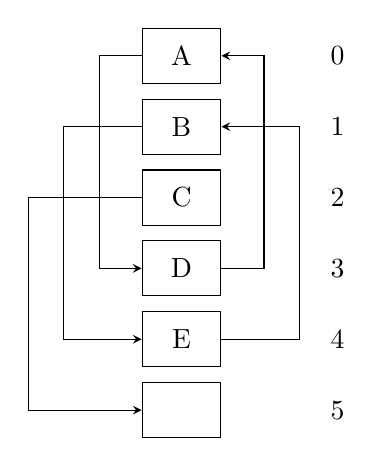
\begin{tikzpicture}[>=stealth,scale=0.9]
  \tikzstyle{slot}=[rectangle,draw,minimum width=1cm,minimum height=0.7cm,inner sep=0pt]

  % Slots (0..5)
  \node[slot] (s0) at (0,0) {A};
  \node[slot] (s1) at (0,-1) {B};
  \node[slot] (s2) at (0,-2) {C};
  \node[slot] (s3) at (0,-3) {D};
  \node[slot] (s4) at (0,-4) {E};
  \node[slot] (s5) at (0,-5) {};

  % Indices
  \node at (2.2,0) {0};
  \node at (2.2,-1) {1};
  \node at (2.2,-2) {2};
  \node at (2.2,-3) {3};
  \node at (2.2,-4) {4};
  \node at (2.2,-5) {5};

  % A <-> D (0 <-> 3)
  \draw[->] (s0.west) -- ++(-0.6,0) |- (s3.west);
  \draw[->] (s3.east) -- ++(0.6,0) |- (s0.east);

  % B <-> E (1 <-> 4)
  \draw[->] (s1.west) -- ++(-1.1,0) |- (s4.west);
  \draw[->] (s4.east) -- ++(1.1,0) |- (s1.east);

  % C <-> (empty) 5  (2 <-> 5)
  \draw[->] (s2.west) -- ++(-1.6,0) |- (s5.west);
\end{tikzpicture}
\end{center}

We now insert a new key \(K\), whose possible positions are
\(h_{1}(K)=3\) and \(h_{2}(K)=2\), using standard cuckoo hashing.
Which hash table do we end up with?

\oneanswer
\optionsstart
\answer \(\langle D, B, K, A, E, C \rangle\) \correct
\answer \(\langle A, B, K, D, E, C \rangle\)
\answer \(\langle D, B, C, K, E, A \rangle\)
\answer \(\langle A, E, K, D, B, C \rangle\)
\answer It is undefined, since an infinite loop will occur during the insertion, so a rehash will take place.
\optionsend
\explanation{
The insertion proceeds as follows:
\begin{itemize}
  \item \(K\) is inserted at position \(3\),
    so \(D\) is evicted to its alternative position \(0\).
  \item \(D\) is inserted at position \(0\),
    so \(A\) is evicted to its alternative position \(3\).
  \item \(A\) is inserted at position \(3\),
    so \(K\) is evicted to its alternative position \(2\).
  \item \(K\) is inserted at position \(2\),
    so \(C\) is evicted to its alternative position \(5\),
        which is empty. Since \(C\) is placed in an empty slot, the insertion stops here.
\end{itemize}
The final table is therefore
\begin{align*}
  \langle D, B, K, A, E, C \rangle.
\end{align*}
}


\question{Matrix computation}
Let
\begin{align*}
    A =
\begin{bmatrix}
1 & 0\\
2 & 1\\
0 & 1
\end{bmatrix}
\quad \text{and} \quad
B =
\begin{bmatrix}
1 & 1\\
0 & 2\\
1 & 0
\end{bmatrix}.
\end{align*}

Compute \(A^{T}B\). Here \(A^{T}\) is the transpose of \(A\).

\oneanswer
\optionsstart
\answer \correct
\(\displaystyle
\begin{bmatrix}
1 & 5\\
1 & 2
\end{bmatrix}\)
\itxanswer{[[1,5],[1,2]]}

\answer \(\displaystyle
\begin{bmatrix}
1 & 1\\
5 & 2
\end{bmatrix}\)
\itxanswer{[[1,1],[5,2]]}

\answer \(\displaystyle
\begin{bmatrix}
1 & 5\\
0 & 3
\end{bmatrix}\)
\itxanswer{[[1,5],[0,3]]}

\answer \(\displaystyle
\begin{bmatrix}
1 & 0\\
5 & 3
\end{bmatrix}\)
\itxanswer{[[1,0],[5,3]]}

\optionsend
\explanation{
We have
\begin{align*}
    A^{T} =
\begin{bmatrix}
1 & 2 & 0\\
0 & 1 & 1
\end{bmatrix}.
\end{align*}

Hence

\begin{align*}
    A^{T}B =
\begin{bmatrix}
1 & 2 & 0\\
0 & 1 & 1
\end{bmatrix}
\begin{bmatrix}
1 & 1\\
0 & 2\\
1 & 0
\end{bmatrix}
=
\begin{bmatrix}
1\cdot1 + 2\cdot0 + 0\cdot1 & 1\cdot1 + 2\cdot2 + 0\cdot0\\
0\cdot1 + 1\cdot0 + 1\cdot1 & 0\cdot1 + 1\cdot2 + 1\cdot0
\end{bmatrix}
=
\begin{bmatrix}
1 & 5\\
1 & 2
\end{bmatrix}.
\end{align*}

}


\question{Dijkstra's algorithm}
Consider the following weighted, directed graph:

\begin{center}
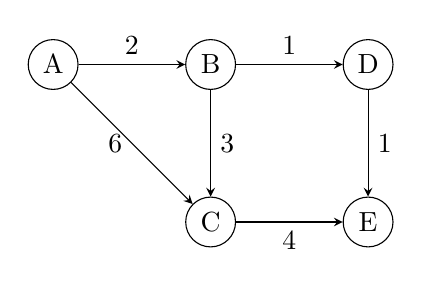
\begin{tikzpicture}[>=stealth, node distance=2.4cm]
  \tikzstyle{vertex}=[circle,draw,minimum size=18pt,inner sep=0pt]

  \node[vertex] (A) at (0,0) {A};
  \node[vertex] (B) at (2,0) {B};
  \node[vertex] (C) at (2,-2) {C};
  \node[vertex] (E) at (4,-2) {E};
  \node[vertex] (D) at (4,0) {D};

  \draw[->] (A) -- node[above] {2} (B);
  \draw[->] (A) -- node[left] {6} (C);
  \draw[->] (B) -- node[right] {3} (C);
  \draw[->] (B) -- node[above] {1} (D);
  \draw[->] (C) -- node[below] {4} (E);
  \draw[->] (D) -- node[right] {1} (E);
\end{tikzpicture}
\end{center}

Suppose Dijkstra's algorithm is used to find shortest paths from vertex \(A\)
to all vertices in the graph.
State the order in which the vertices are extracted from
the priority queue in Dijkstra's algorithm.
\oneanswer

\optionsstart
\answer \(A C B D E\)
\answer \(A C E B D\)
\answer \(A B C D E\)
\answer \(A B D E C\) \correct
\optionsend
\explanation{
  \begin{itemize}
      \item Start: \(d(A)=0\), all others \(\infty\).
      \item From \(A\): \(d(B)=2\), \(d(C)=6\). The next vertex is \(B\) (smallest distance).
\item From \(B\): \(d(C)\) is improved to \(2+3=5\), \(d(D)=2+1=3\).
\item The next vertex is \(D\) (distance \(3\)), which gives \(d(E)=3+1=4\).
\item The next vertex is \(E\) (distance \(4\)).
\item The last vertex is \(C\) (distance \(5\)).
\end{itemize}
The order is therefore \(A,B,D,E,C\).
}






\multiplechoiceend

\label{page:last}
